\section{DNA}
\label{sec:dna}

L'essenza della vita risiede nell'intricata danza del DNA, o acido desossiribonucleico, una molecola situata nel nucleo di ogni cellula. Tale molecola è, in realtà, una macro-molecola e si identifica facilmente nella caratteristica forma a doppia elica costituita da due catene nucleotidiche. Ogni nucleotide che compone la catena è costituito da una molecola di zucchero-fosfato e da una base azotata. Riconosciamo quattro basi azotate, Adenina, Citosina, Guanina e Timina, che si legano a due a due attraverso legami idrogeno formando delle coppie specifiche, come illustrato in Figura~\ref{fig:DNA-double-helix-structure}: Adenina e Timina (A-T), Citosina e Guanina (C-G). L'ordine con cui si susseguono le basi azotate lungo la catena nucleotidica orchestra la sinfonia dell'esistenza.

\begin{figure}[!ht]
	\centering
	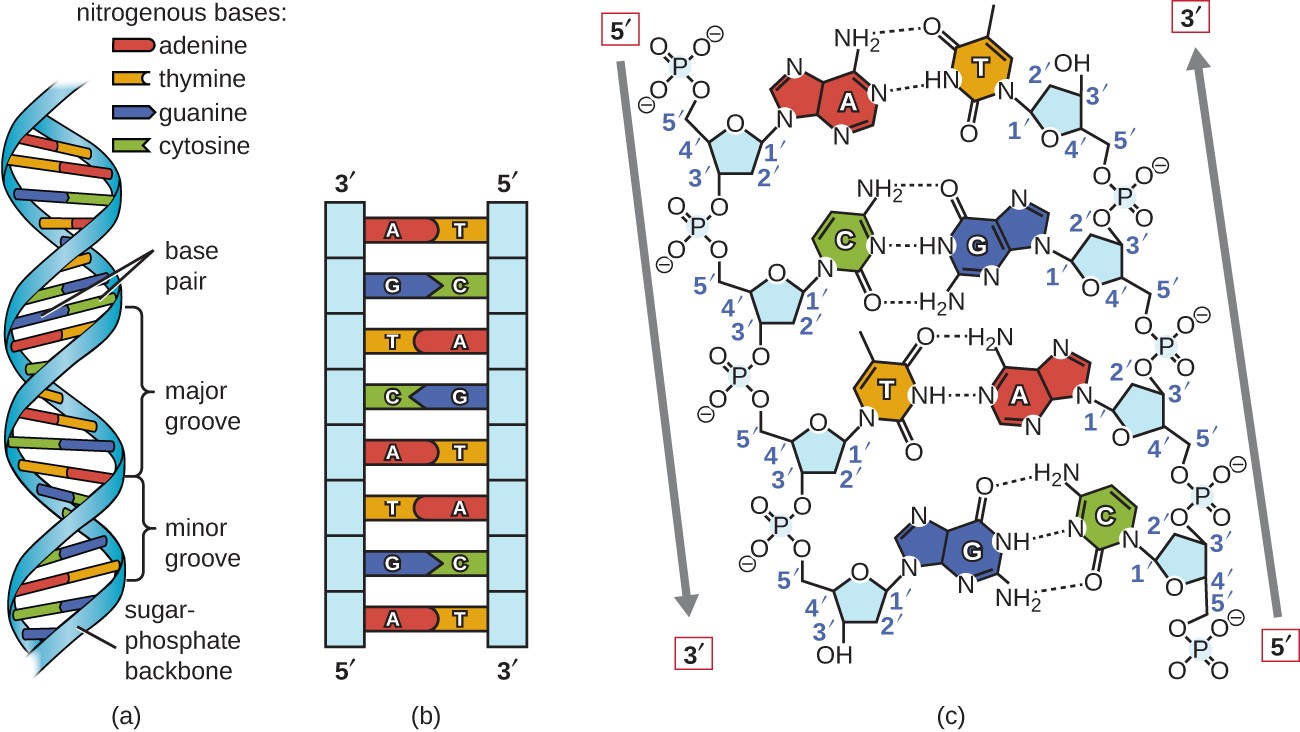
\includegraphics[width=0.85\linewidth]{images/dna-structure}
	\caption{The fundamental structure of the \acs{DNA} double helix consists of two strands, each composed of chains of nucleotides. Within this framework, every nucleotide forms a bond with its complementary counterpart on the opposing strand \cite{openstax_microbiology_2016}.}
	\label{fig:DNA-double-helix-structure}
\end{figure}




\subsection{DNA sequencing}
\label{subsec:dna-sequencing}

Il sequenziamento del DNA è il processo di determinazione della sequenza nucleotidica di un frammento di DNA, ed è fondamentale per la ricerca genetica, la biologia molecolare, la medicina e altre discipline. Sono state numerose le tecnologie sviluppate nel corso degli anni per rendere questo processo più veloce, preciso e accessibile. Anche i costi sono diminuiti drasticamente: dal Progetto Genoma Umano, che ha richiesto miliardi di dollari, siamo passati a tecnologie che permettono il sequenziamento di un intero genoma umano per meno di 1.000 dollari. Il costo, ovviamente, varia a seconda della tecnologia utilizzata, della copertura richiesta e della complessità del progetto. Le piattaforme NGS come Illumina e Ion Torrent offrono opzioni economiche per progetti su larga scala, mentre tecnologie come PacBio, pur essendo più costose, forniscono dettagli unici per esigenze specifiche. Di seguito, vengono descritte le principali tecniche di sequenziamento.

\begin{figure}[!ht]
	\centering
	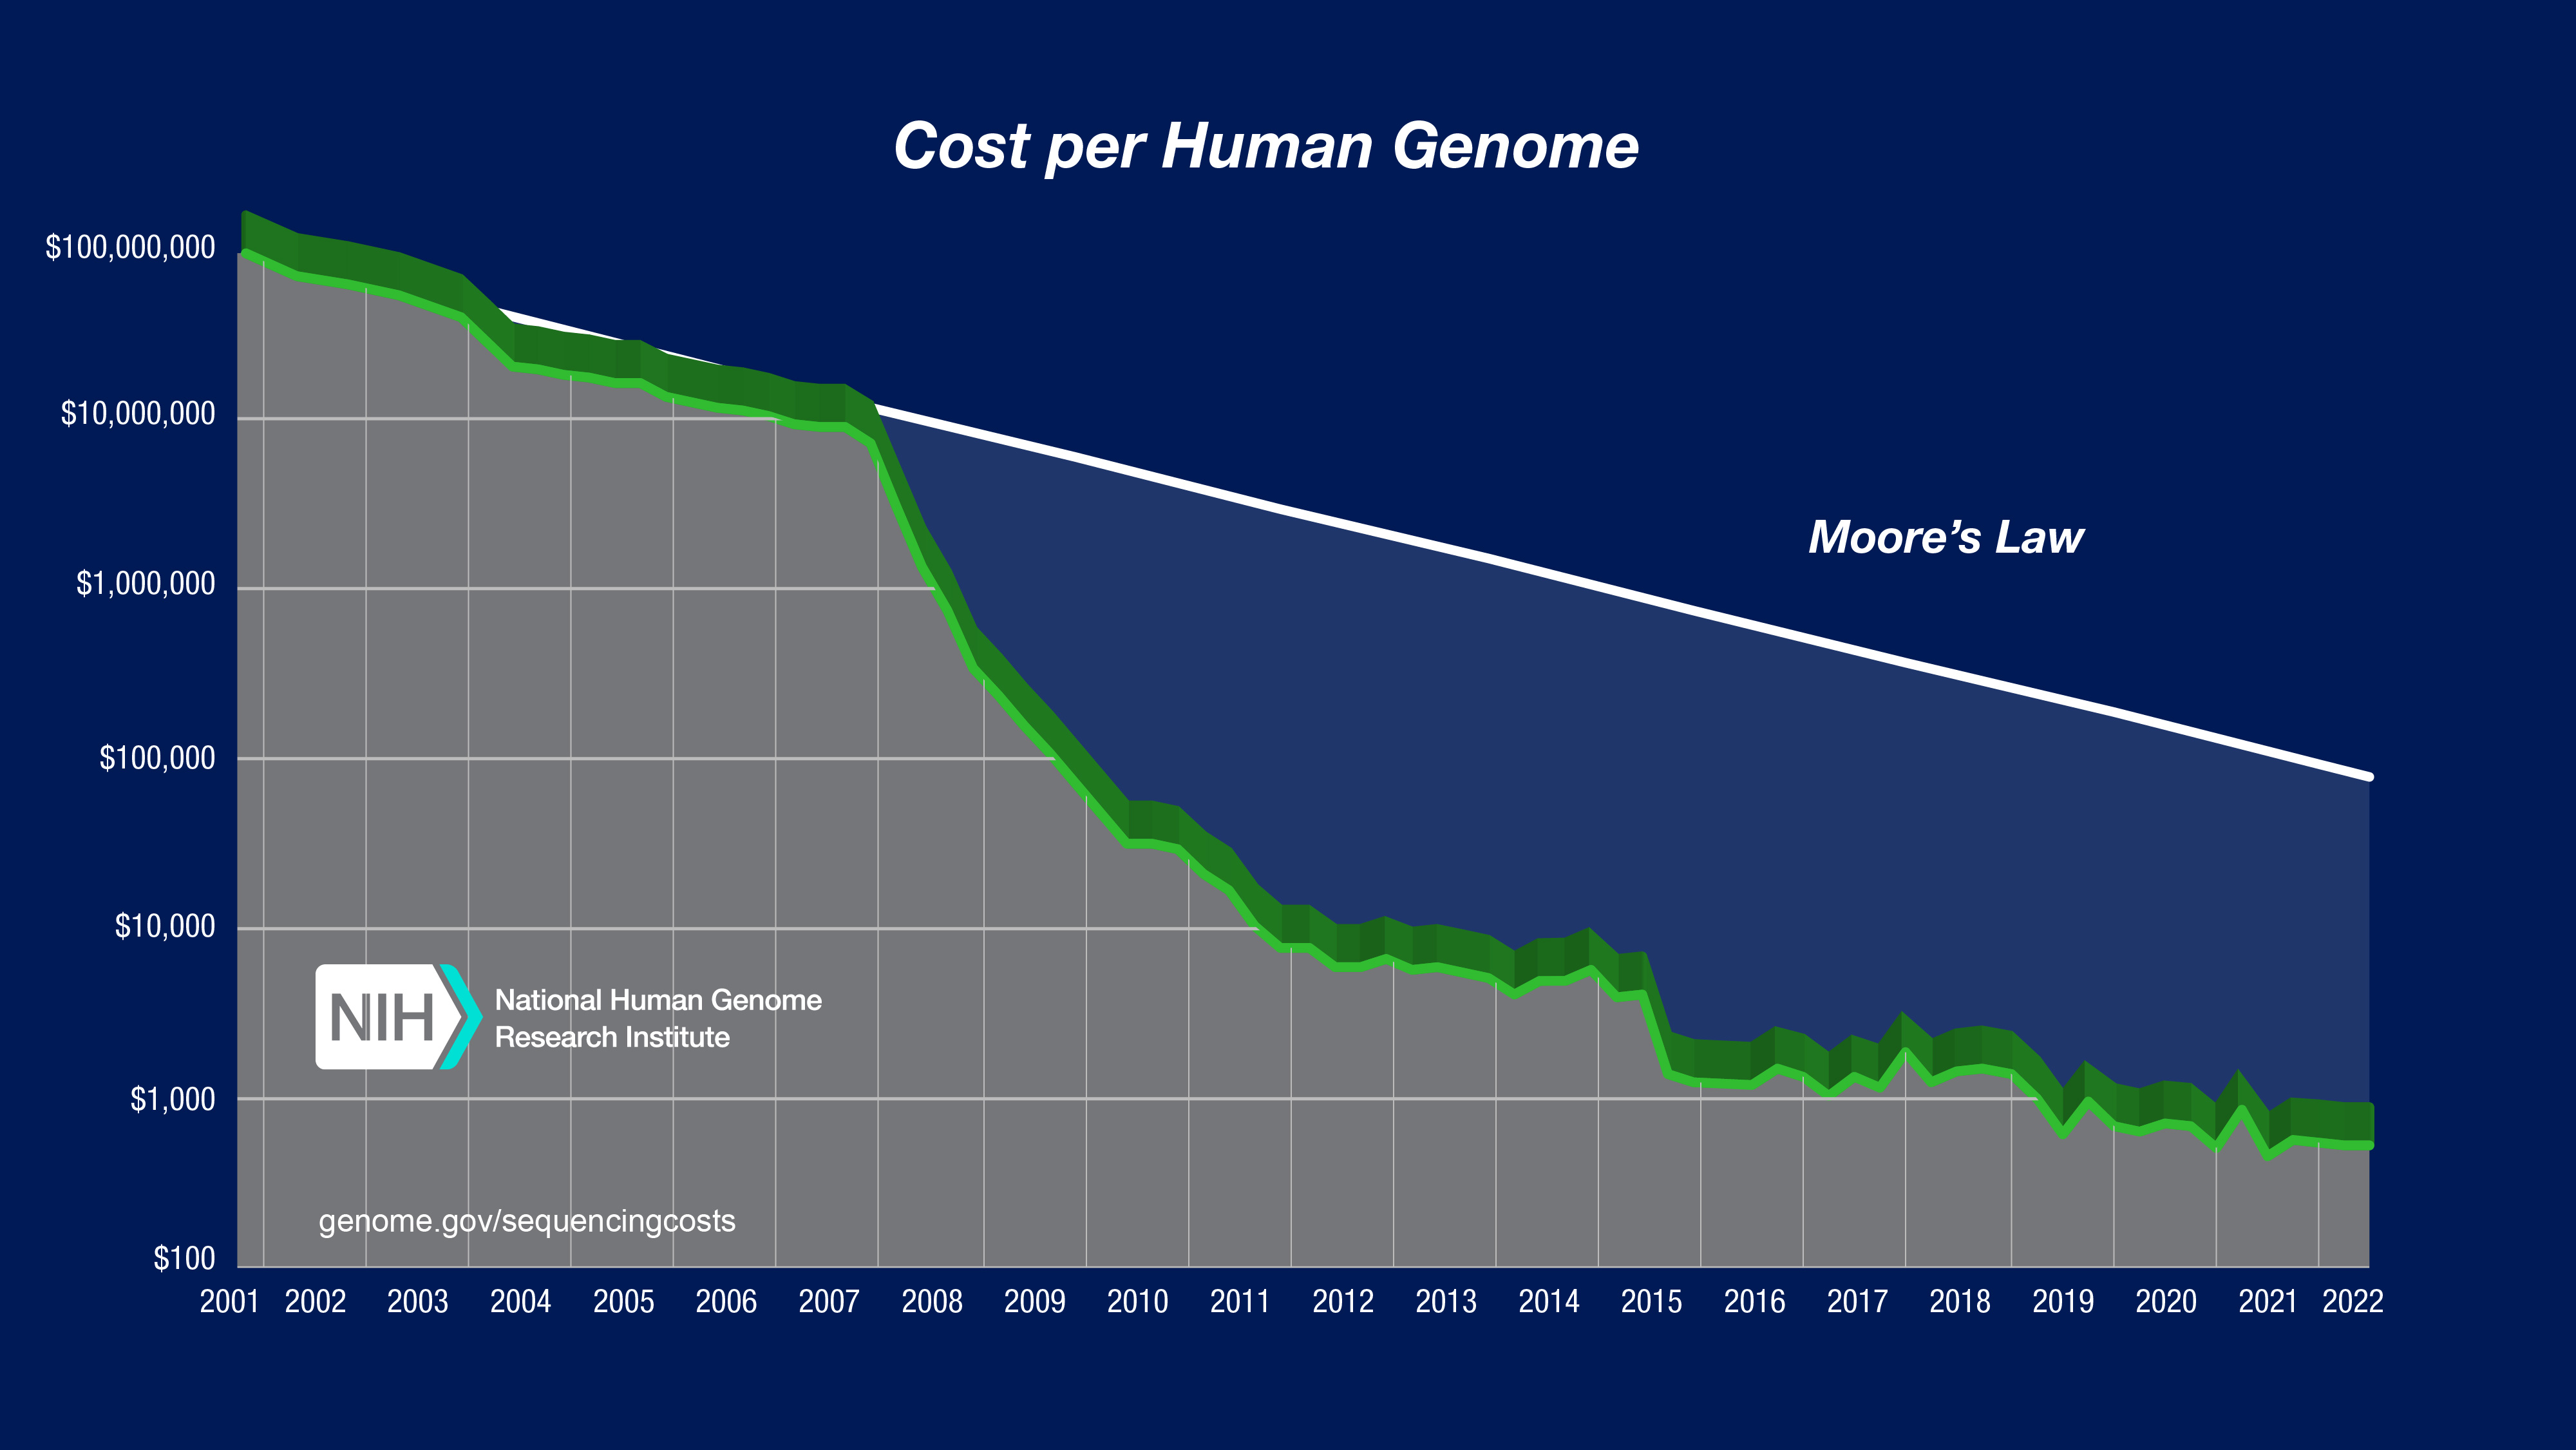
\includegraphics[width=0.85\linewidth]{images/2022_Sequencing_cost_per_Human_Genome}
	\caption{Sequencing cost per genome data - 2022: the cost per genome has become much lower than Moore’s Law \cite{cost_sequencing}.}
	\label{fig:sequencing-cost-per-human-genome}
\end{figure}

\begin{figure}[!ht]
	\centering
	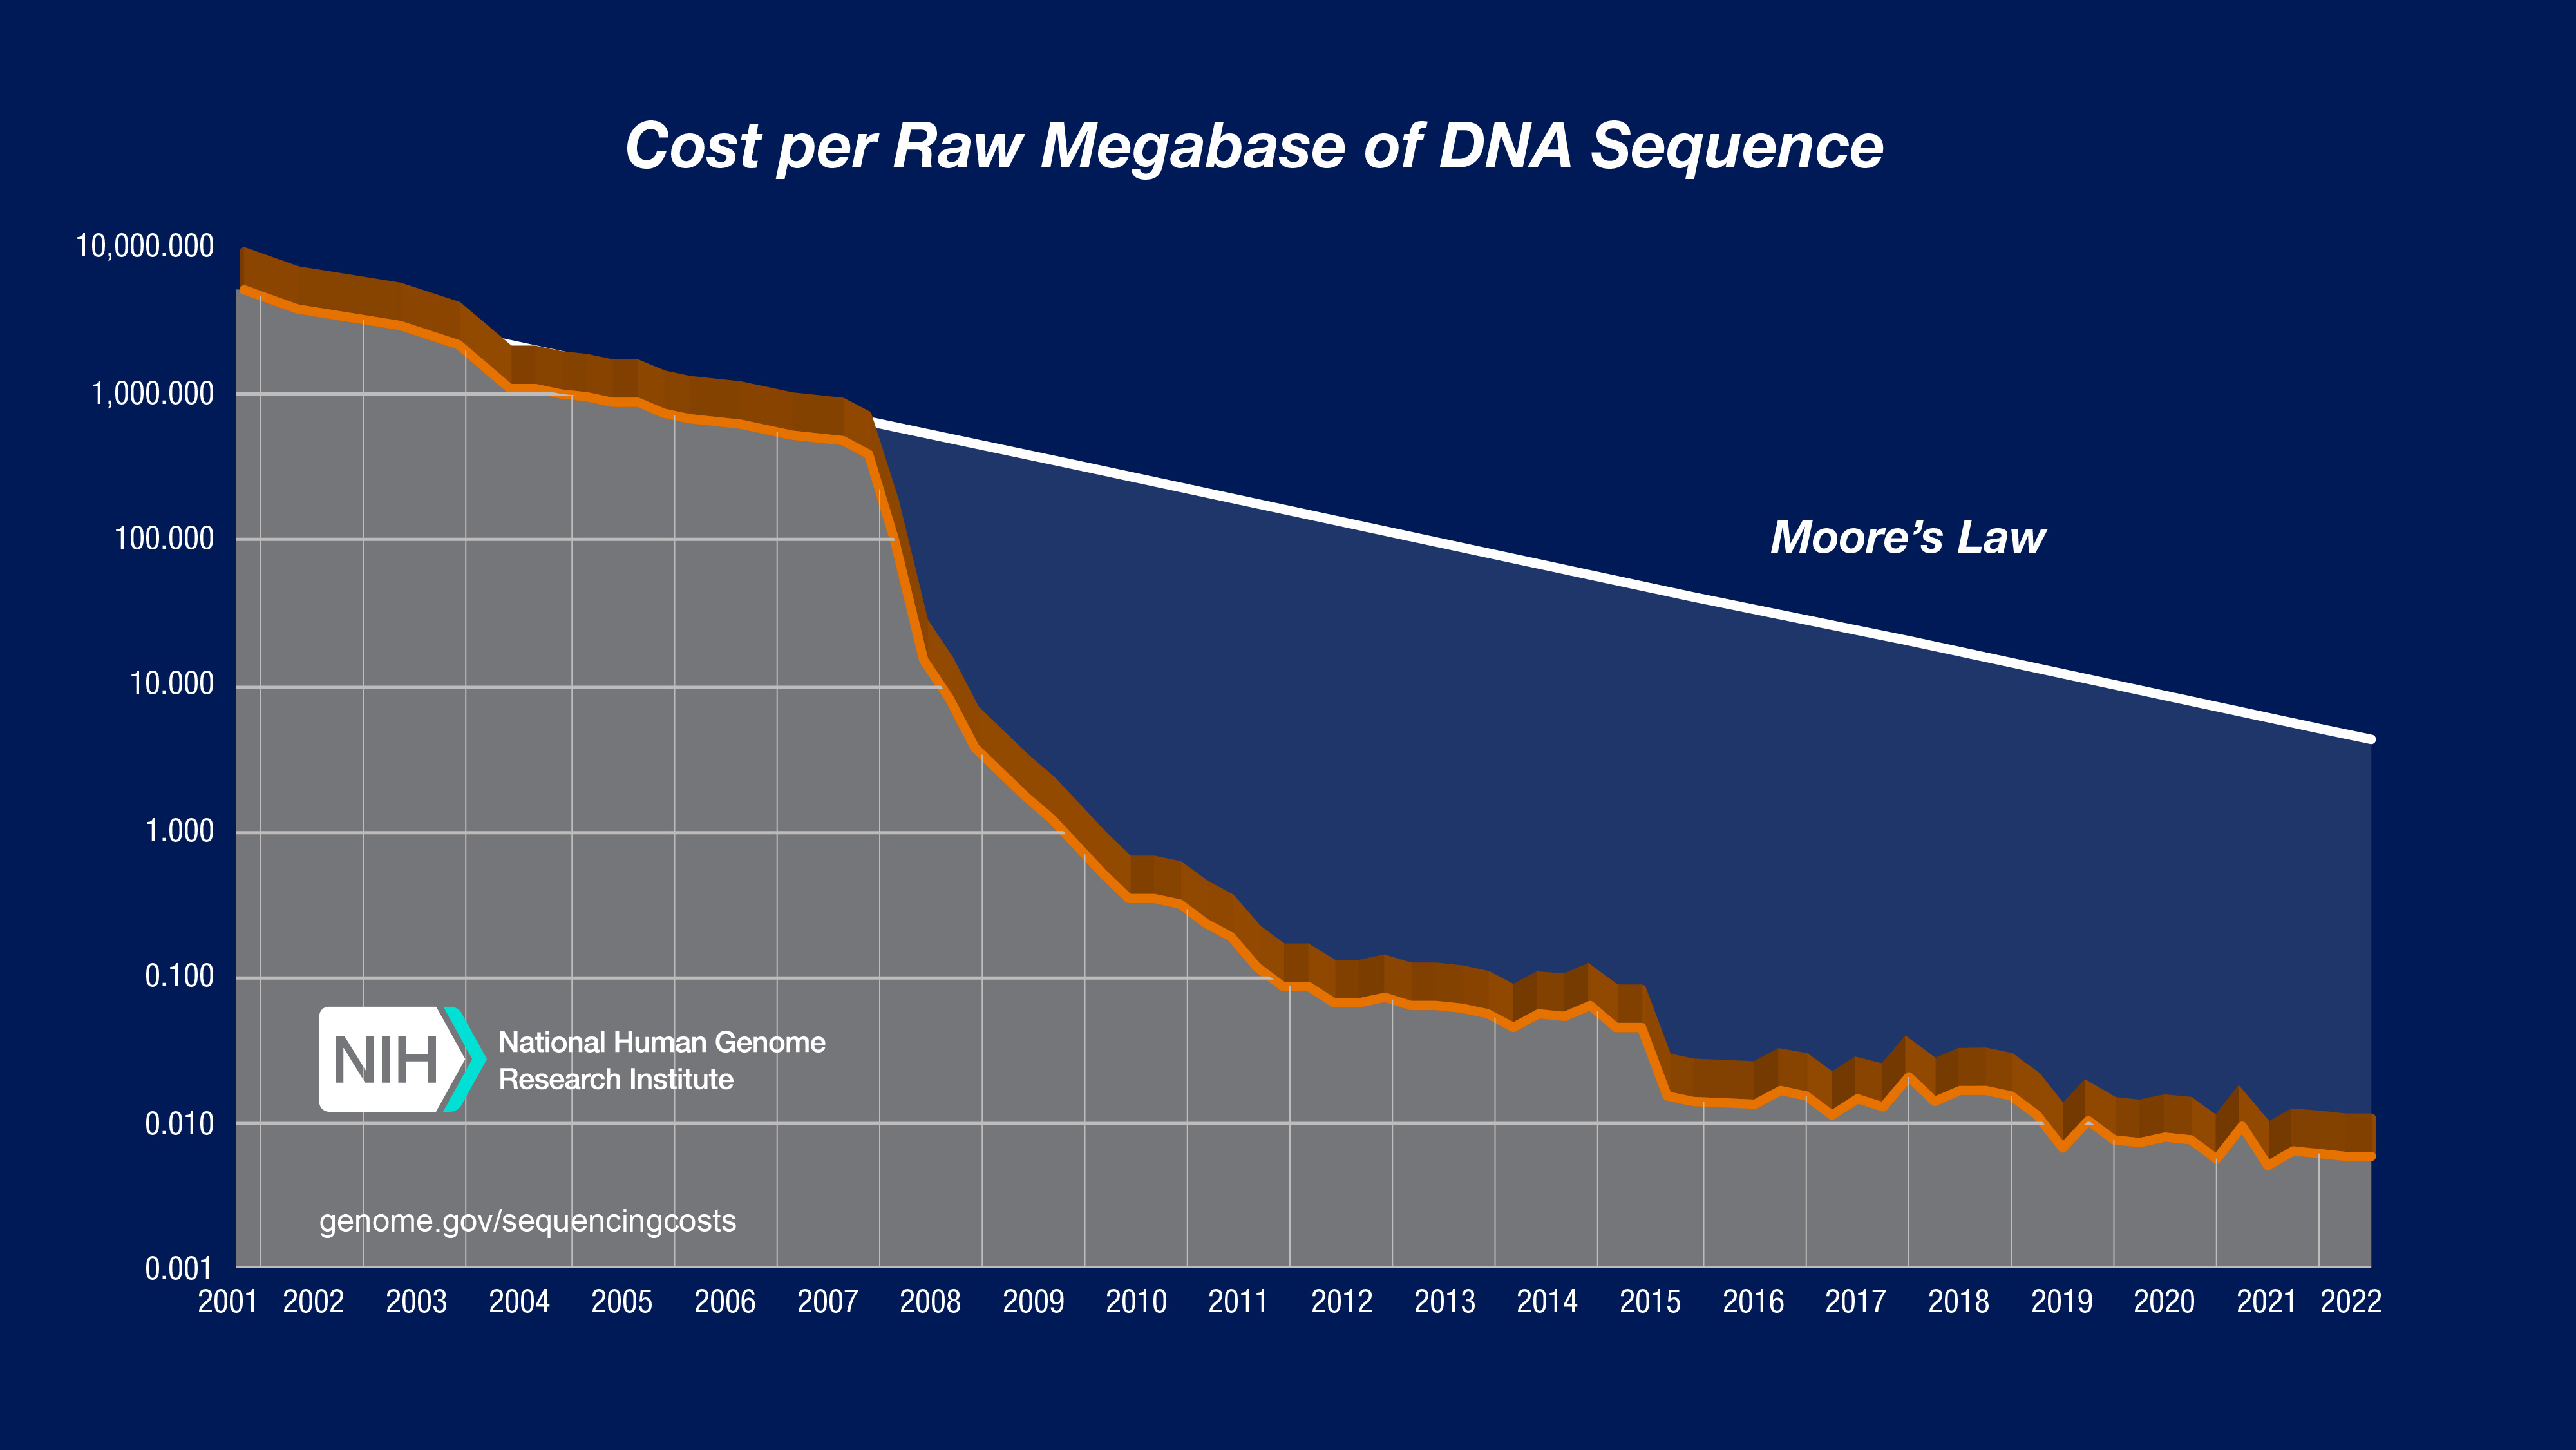
\includegraphics[width=0.85\linewidth]{images/2022_Sequencing_cost_per_Mb}
	\caption{Sequencing cost per megabase - 2022: the cost per megabase has become much lower than Moore’s Law \cite{cost_sequencing}.}
	\label{fig:sequencing-cost-per-mb}
\end{figure}


	\subsubsection{Sanger Method}
	Il metodo Sanger, sviluppato da Frederick Sanger negli anni '70, è stato il primo approccio di successo per il sequenziamento del DNA. Utilizza la terminazione della catena, dove dideossinucleotidi (ddNTP) interrompono la sintesi del DNA, permettendo la lettura della sequenza in base alla lunghezza dei frammenti ottenuti. Sebbene sia preciso, il metodo Sanger è relativamente lento e costoso, adatto principalmente a sequenze di DNA più corte. Questo metodo è stato utilizzato per il Progetto Genoma Umano, che ha sequenziato l'intero genoma umano a un costo di circa 2,7 miliardi di dollari.
	
	\subsubsection{Next-Generation Sequencing}
	Negli ultimi decenni, le tecnologie di Next-Generation Sequencing (NGS) hanno rivoluzionato il campo, permettendo il sequenziamento massivo e parallelo di miliardi di frammenti di DNA. Tra le piattaforme NGS, spiccano Illumina, Ion Torrent e PacBio.
	
	\begin{figure}[!ht]
		\centering
		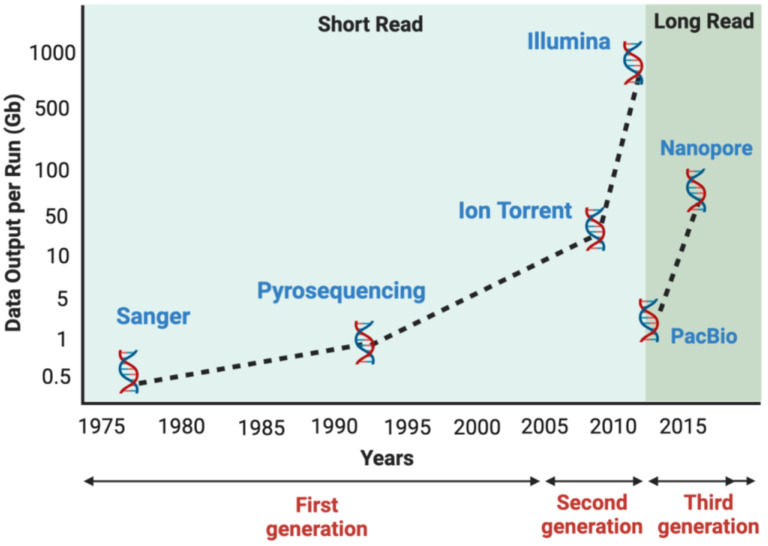
\includegraphics[width=0.85\linewidth]{images/next-generation_sequencing_technology}
		\caption{Evolution of sequencing technologies \cite{ngs-technologies}.}
		\label{fig:evolution-sequencing-technologies}
	\end{figure}
	

	Illumina è uno dei leader nel mercato NGS. Utilizza la tecnologia di sequenziamento per sintesi (SBS), dove i nucleotidi marcati con fluorescenza vengono incorporati nel DNA, e le immagini fluorescenti rivelano la sequenza. Questo metodo offre alta accuratezza e profondità di lettura, rendendolo ideale per progetti di genomica su larga scala. Il costo per sequenziare un genoma umano completo con Illumina può variare da poche centinaia a qualche migliaio di dollari, a seconda della copertura e delle specifiche del progetto.
	
	La tecnologia Ion Torrent, sviluppata da Life Technologies, si basa sulla rilevazione del rilascio di ioni idrogeno durante l'incorporazione dei nucleotidi. Questo approccio senza fluorescenza permette un sequenziamento rapido e a basso costo. Sebbene l'accuratezza possa essere inferiore rispetto a Illumina, Ion Torrent è vantaggioso per applicazioni che richiedono velocità e costi ridotti.
	
	Pacific Biosciences (PacBio) ha introdotto la tecnologia Single Molecule Real-Time Sequencing (SMRT). Offre la capacità di leggere lunghe sequenze di DNA, con letture che possono superare i 10.000 basi. Questo è particolarmente utile per l'assemblaggio \emph{De Novo} di genomi, ma anche per l'analisi di complesse regioni ripetitive. Nonostante i costi più elevati rispetto ad altre tecnologie NGS, PacBio è utile per studi che richiedono letture lunghe e dettagliate.



	\subsection{Assembly Techniques}
	\label{subsec:assembly-techniques}
	
	Il sequenziamento del DNA produce frammenti, chiamati read, che devono essere assemblati per ricostruire la sequenza originale. Queste le due principali strategie di assemblaggio:
	\begin{itemize}
		\item L'assemblaggio De Novo viene utilizzato quando non si dispone di una sequenza di riferimento. I frammenti vengono assemblati basandosi solo sulle sovrapposizioni tra di essi. Questa tecnica è fondamentale per sequenziare nuovi genomi.
		
		\item Nell'assemblaggio Reference, usato principalmente per studi di variabilità genetica, i frammenti vengono allineati a una sequenza di riferimento esistente. Questo facilita il processo di assemblaggio e migliora l'accuratezza.
	\end{itemize}
